\chapter{Introduction}

Typical programming languages are defined in terms of plaintext tokens. These tokens
are then used in grammar rules to specify which orderings of tokens are valid programs and
which are not.
\begin{figure}[!hbt]
	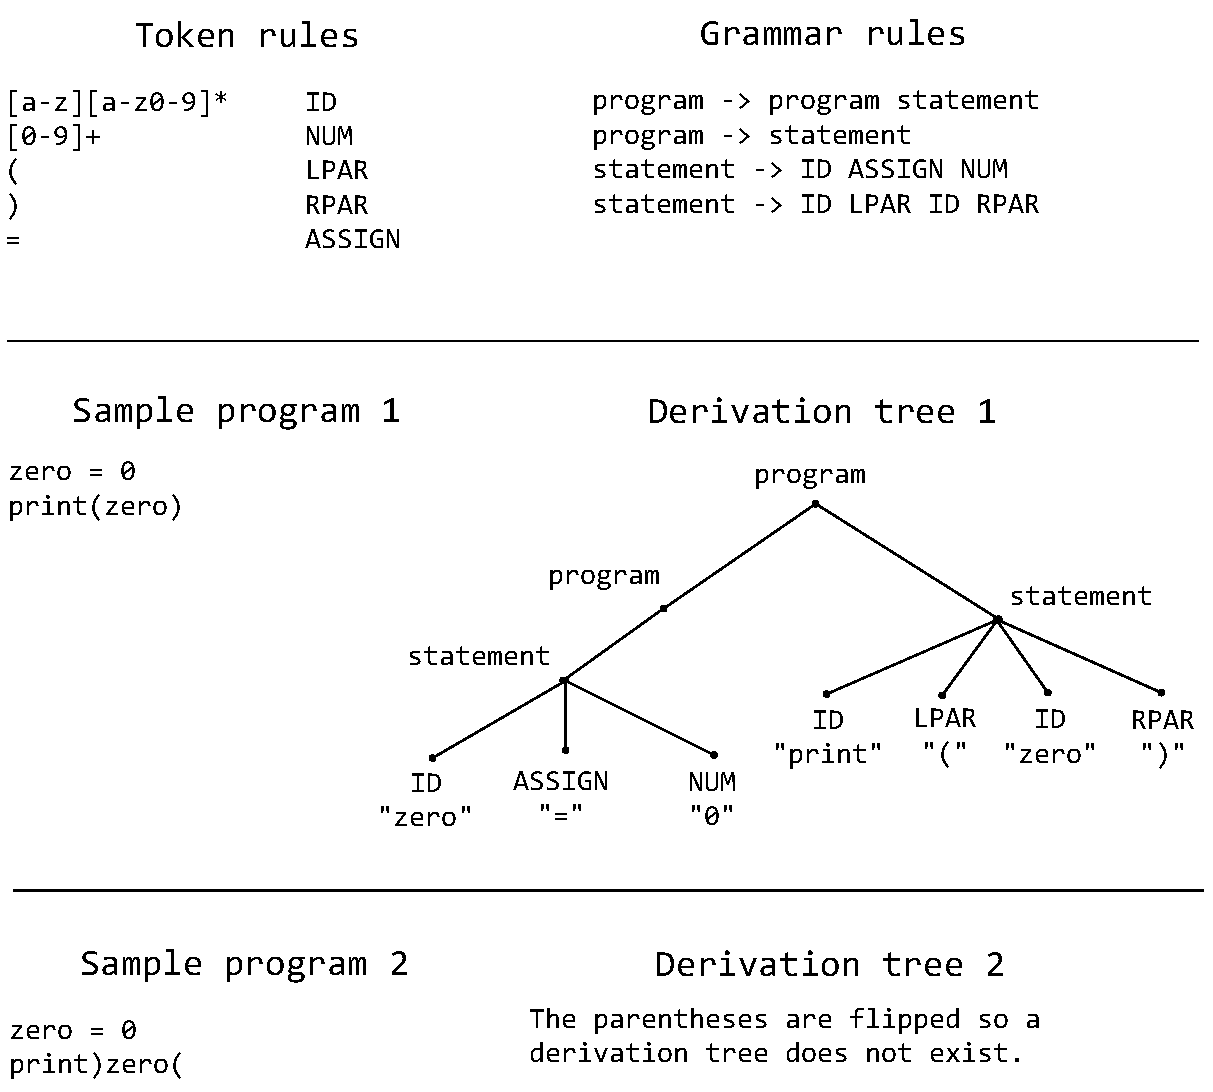
\includegraphics[width=\textwidth]{../img/tokens_and_grammar}
	\caption{Sample language definition with examples}
	\label{fig:chap1:tokens_and_grammar}
\end{figure}

On the figure \ref{fig:chap1:tokens_and_grammar} we see a set of token rules and grammar rules defining a~simple
language. Sample program $1$ shows a valid program in this language with its respective derivation tree, while
second program does not adhere to the defined grammar rules.
While given example is trivial it shows how vast majority of programming languages are defined and processed:
\begin{itemize}
\item Users write plaintext source code
\item Lexical analysis splits the source code into tokens based on the rules provided
\item Syntax analysis builds a tree (AST or derivation tree) based on the grammar rules
\item AST is used to compile, interpret or transpile the source code
\end{itemize}

However, tokens do not have to consist of plaintext necessarily. Plaintext characters can be substituted for
images, videos, sounds, etc. In this thesis we construct a programming language with characters and some
of the tokens substituted for images or short looping videos (e.g. GIFs). A Figure \ref{fig:chap1:giflang_code} below shows
the Sample program 1 from \ref{fig:chap1:tokens_and_grammar} written in Giflang\footnote{We named the programming
language developed in this thesis Giflang}.
\begin{figure}[!hbt]
	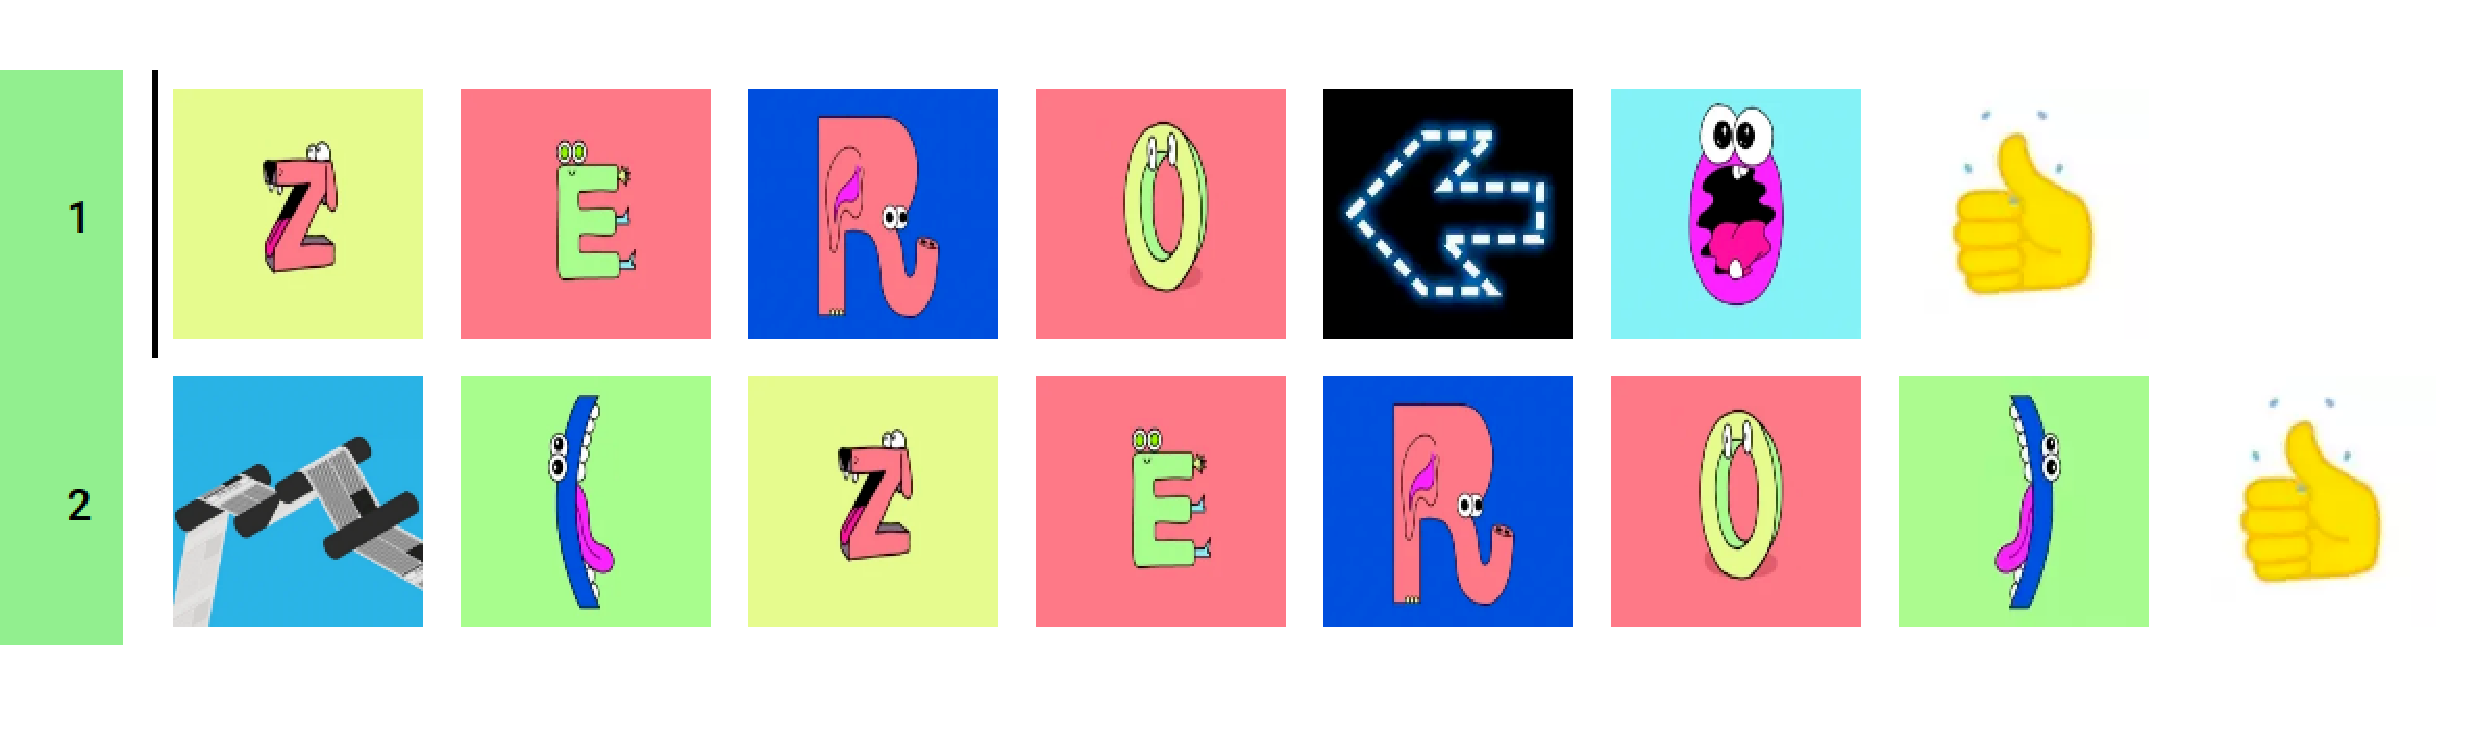
\includegraphics[width=\textwidth]{../img/giflang_code}
	\caption{Sample code in Giflang}
	\label{fig:chap1:giflang_code}
\end{figure}

You can see that characters and digits have their counterparts in Giflang. Assignment is represented with an arrow,
thumbs up is a semicolon and `print' function is a single image containing paper. The exact choice of images used here is of course
not very relevant.

In order to be able to store and parse programs like that we also need to define an intermediate
format. The format can be for example textual and the sample program from Figure \ref{fig:chap1:giflang_code} can be written as:
\begin{code}
Z;E;R;O; ASSIGN; 0; SEMICOLON;
PRINT; LPAR; Z;E;R;O; RPAR; SEMICOLON;
\end{code}

We actually chose the format shown above. We discuss the intermediate format and the language design in section /TODO/.

You can see that there is a clear mapping between images and semicolon-delimited tokens. Therefore, a byproduct of
this thesis is a token-level programming language, i.e. a language that consists of delimited tokens. This tokens
can have different presentational forms as mentioned before.

A language like this one is of course impractical and hard to follow. We do not intend to create a language
for practical use. Our $3$ main motivations for creating Giflang are:
\begin{enumerate}
\item An image-based programming language like this does not exist yet. We discuss other existing visually oriented
languages in section /TODO/. 
\item Using it in bootcamps for elementary and high schoolers. We co-organize a long-term Computer Science competition
named Prask\footnote{prask.ksp.sk todo}. After each semester we invite best contestants to a week-long bootcamp
filled with creative games mostly related to Computer Science. Giflang can be used as part of the games.
\item Allowing users to substitute images for their own can give younger users feeling of creating ''their own language''.
\end{enumerate}

Since we use images instead of characters we need to implement our own IDE to be able to create and run Giflang programs. Typically,
IDEs are desktop applications. However, since ease of access and use have bigger priority than efficiency for this application
we decided to move everything to a browser.

To sum up it up, in this thesis we design a programming language with characters and some of the tokens substituted for images.
Additionally, we build an interpreter and an IDE for this language that both run in browser. Goals mentioned here are described
more precisely in the Section \ref{chap1:thesis_goals}. 

\section{Related work}
\cite{Andel07}
Visual programming languages have been around since ... and this thesis was undeniably inspired by them. A visual 
programming language lets users create programs by manipulating program elements graphically rather than by specifying them textually\footnote{Wikipedia}.
Giflang is not a visual programming language as users can not manipulate with graphics in its IDE, e.g. move it, connect it with other
objects, etc. It is also not a textual language per-se as text is replaced by images. However, it is definitely closer to a textual
rather than a visual programming language so we could say that it is a semi-textual programming language.

This section will discuss programming languages we got inspired from and also multiple web IDEs since we implement
Giflang for web.

\subsection{Emojicode}
An excerpt from the official documentation: Emojicode is an open source, high-level, multi-paradigm programming language consisting of emojis.
It features Object-Orientation, Optionals, Generics and Closures.

Here is a `Hello World' program in Emojicode:
\begin{figure}[!hbt]
	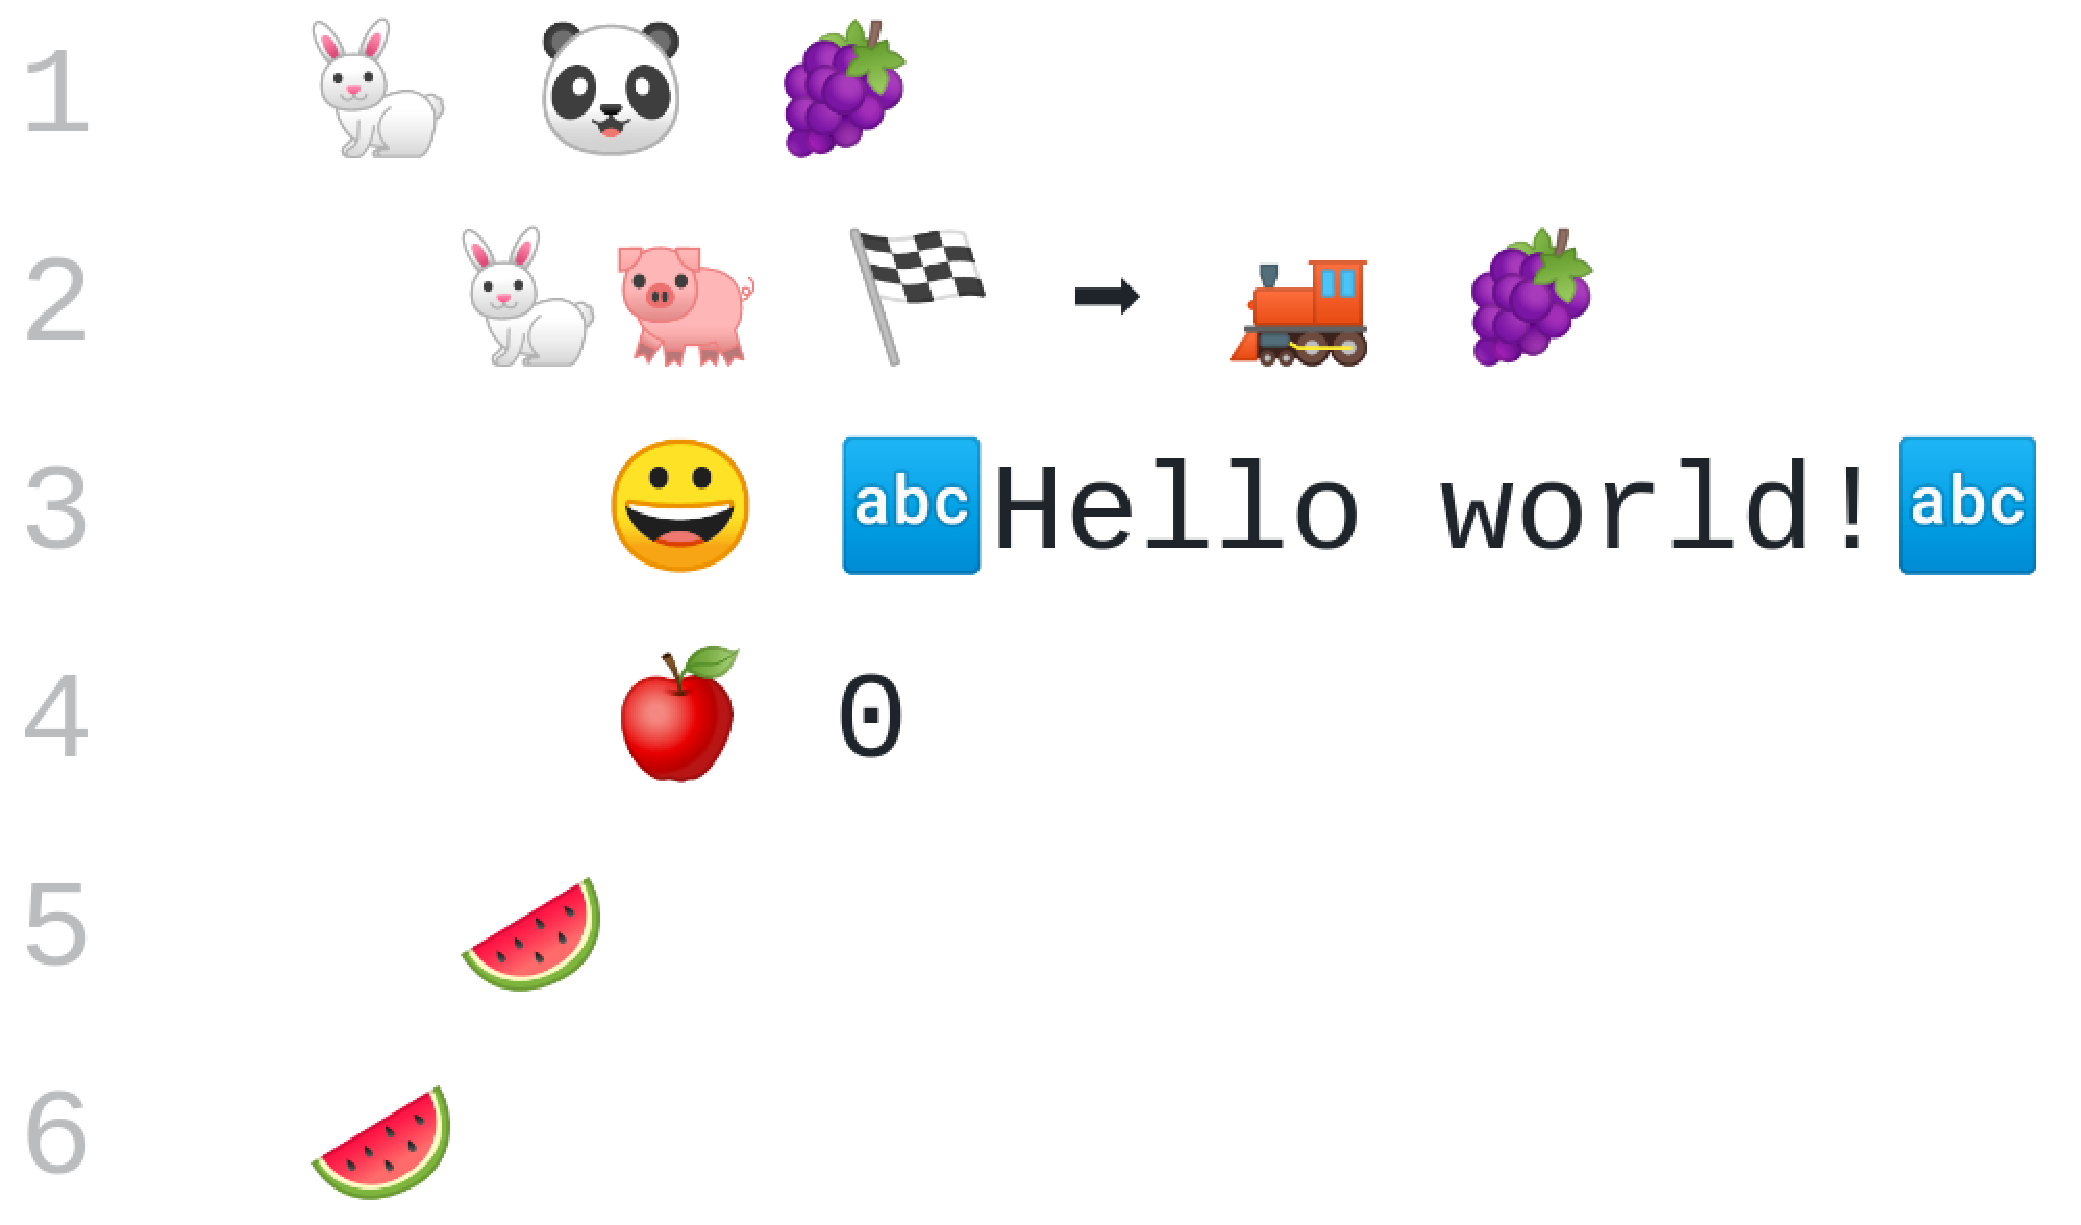
\includegraphics[width=0.5\textwidth]{../img/emojicode_helloworld}
	\label{fig:chap1:emojicode_helloworld}
\end{figure}

All built-in keywords and most of the special characters are replaced by emojis. For example a raspberry is an opening curly brace `{' in Emojicode.
However, as you can on the `Hello World' program not every character is replaced by an emoji. Additionally, users can not create their own emoji
mappings to keywords or characters. Creating Emojicode sources is simple as emojis are just Unicode characters and most of the modern text editors
have a good support for them.

For compilation Emojicode uses LLVM which is a collection of reusable compiler technologies. Source code is compiled first to LLVM IR\footnote{IR or
Intermediate Language is a low-level programming language similar to assembly.} and then to machine code. With features as compilation to an intermediate
language, object-orientation, static typing and garbage collection we can say Emojicode is similar to languages like C\# or Java.

Emojicode is the closest language to the one we build in this thesis. However, since we are replacing characters and keywords with arbitrary images as
opposed to emojis we have to use an intermediate textual format that maps to the images. Emojicode does not have this problem since emojis are
Unicode characters that can be represented in plaintext and parsed.

\subsection{Karel?}
\subsection{REPl?}

\section{IDE as desktop vs browser application}

\section{Thesis goals}
\label{chap1:thesis_goals}